\documentclass{zjureport}
\special{dvipdfmx:config z 0} % 取消PDF压缩,加快速度,最终版本生成的时候最好把这句话注释掉

% =============================================
% Part 0 Edit the info
% =============================================

\major{信息工程}
\name{何铭源}
\partner{焦正浩}
\title{本科实验报告}
\stuid{3240104481}
\college{信息与电子工程学院}
\date{\today}
\lab{东4-421}
\course{电子工程训练(甲)}
\instructor{金向东}
\grades{}
\expname{电子工训基础部分内容}
\exptype{}
\setlength{\parindent}{2em}

\begin{document}
% =============================================
% Part 1 Header
% =============================================
\makecover

% \makecontent

\makeheader

% =============================================
% Part 2
% =============================================
\section{常用电子仪器的使用}
\subsection{万用表的使用练习}
取3个不同阻值的电阻,用万用表测量阻值大小并计算误差。
\begin{table}[H]
  \centering
  \caption{电阻读取}
  \begin{tabular}{C{.3\textwidth}C{.3\textwidth}C{.3\textwidth}}
  \toprule
  读取值  & 测量值  & 计算误差 \\
  \midrule
  10000$\Omega$  & 10001$\Omega$  & 0.01\%  \\
  100$\Omega$    & 100.4$\Omega$  & 0.40\%  \\
  100k$\Omega$ & 100.25k$\Omega$ & 0.25\%  \\
  \bottomrule
  \end{tabular}
\end{table}


取3个不同电容值不同的电容,用万用表测量电容值大小并计算误差。
\begin{table}[H]
  \centering
  \caption{电容读取}
  \begin{tabular}{C{.3\textwidth}C{.3\textwidth}C{.3\textwidth}}
  \toprule
  读取值  & 测量值  & 计算误差 \\
  \midrule
  1$\mu$F  & 1.1066$\mu$F  & 10.66\%  \\
  47$\mu$F    & 59.9$\mu$F  & 27.45\%  \\
  1000pF & 1.044$\mu$F & 4.40\%  \\
  \bottomrule
  \end{tabular}
\end{table}

通过万用表二极管测量挡位测量二极管,二极管带有色环一段为负极,导通压降为\textbf{0.618V}。

通过万用表三极管挡位测试三极管管脚。三极管管脚如图(\ref{三极管})所示,hFE测得为\textbf{358}
\begin{figure}[H]
  \centering
  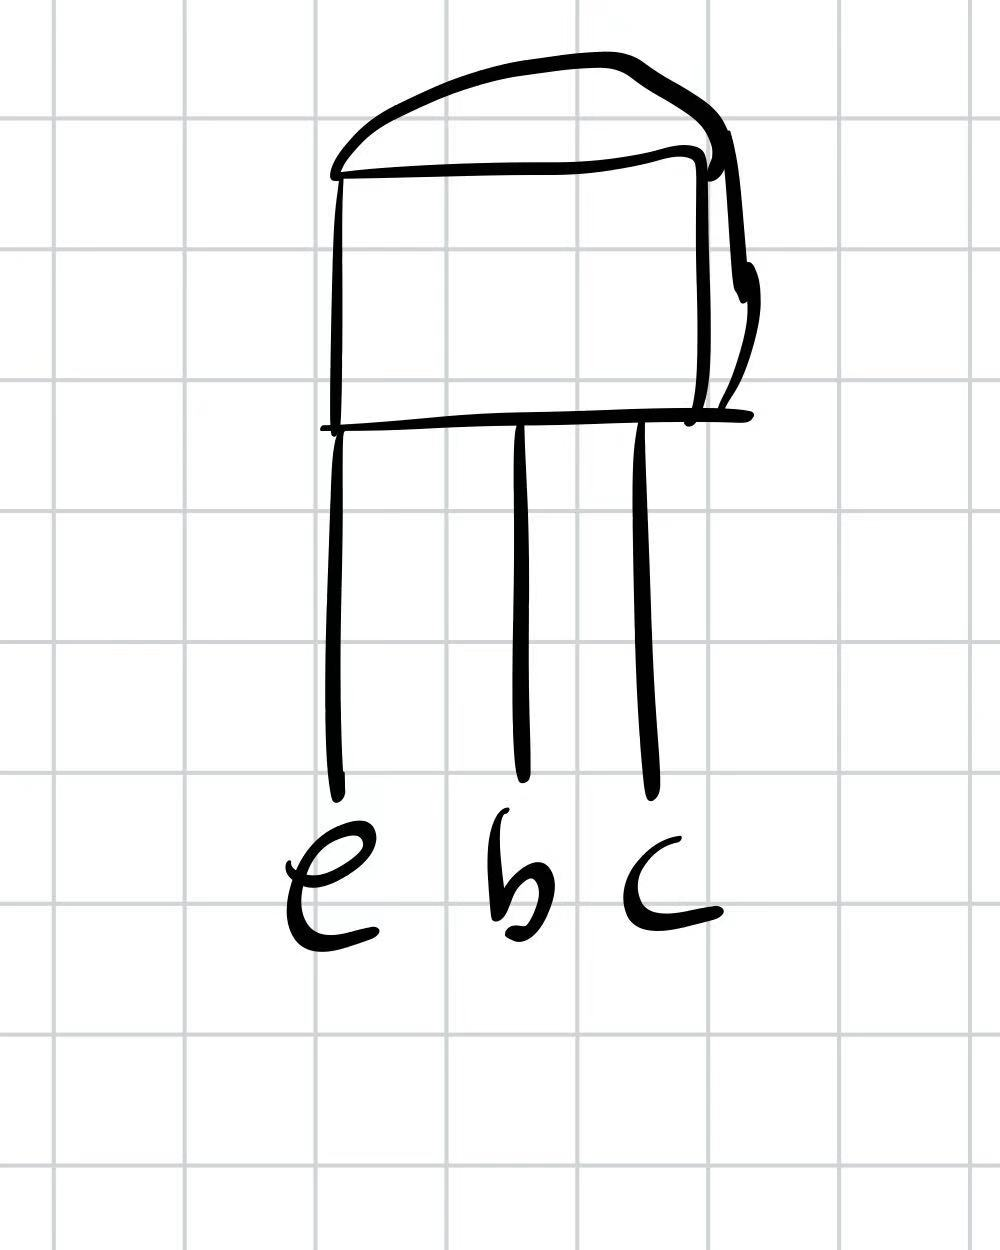
\includegraphics[width = .2\textwidth]{./figures/微信图片_20250318110322.jpg}
  \caption{三极管管脚示意图}
  \label{三极管}
\end{figure}

\subsection{电源与万用表使用练习}
通过设定电源CH1,CH2不同电压大小,并用万用表直流电压档进行测量。
\begin{table}[H]
  \centering
  \caption{电源电压测量}
  \begin{tabular}{C{.3\textwidth}C{.3\textwidth}C{.3\textwidth}}
  \toprule
  设定值  & 测量值  & 计算误差 \\
  \midrule
  12V  & 12.087V  & 0.72\%  \\
  5V    & 5.088V  & 1.76\%  \\
  \bottomrule
  \end{tabular}
\end{table}

设定为串联模式后得到负电压,其中两电源中间串联部分电压为0V。
\begin{table}[H]
  \centering
  \caption{负电压测量}
  \begin{tabular}{C{.3\textwidth}C{.3\textwidth}C{.3\textwidth}}
  \toprule
  设定值  & 测量值  & 计算误差 \\
  \midrule
  $\pm$12V  & 24.096V  & 0.40\%  \\
  $\pm$5V    & 10.202V  & 2.02\%  \\
  \bottomrule
  \end{tabular}
\end{table}

设定限定电流0.5A,电压1.0V,通过万用表2A直流电流挡测量。
\begin{table}[H]
  \centering
  \caption{电源电流测量}
  \begin{tabular}{C{.3\textwidth}C{.3\textwidth}C{.3\textwidth}}
  \toprule
  设定值  & 测量值  & 计算误差 \\
  \midrule
  0.5A  & 0.5080A  & 1.60\%  \\
  \bottomrule
  \end{tabular}
\end{table}

\subsection{信号源与示波器使用练习}
使用Autoset键观察校准信号源波形,并用Cursor模式计算信号幅度。
\begin{table}[H]
  \centering
  \caption{用光标法测量信号的幅度}
  \begin{tabular}{C{.3\textwidth}C{.3\textwidth}C{.3\textwidth}}
  \toprule
  光标Y1  & 光标Y2  & Y1-Y2 \\
  \midrule
  248mV & -264mV  & 512mV \\
  \bottomrule
  \end{tabular}
\end{table}
调节信号源幅度为0.2Vp-p,频率依次为10kHz,100kHz,1MHz,测量输出的正弦波峰值和频率。
\begin{table}[H]
  \centering
  \caption{调节信号源}
  \begin{tabular}{C{.4\textwidth}C{.4\textwidth}}
  \toprule
  峰值  & 频率 \\
  \midrule
  206mV & 10.00kHz \\
  202mV & 99.28kHZ \\
  208mV & 1.006MHz \\
  \bottomrule
  \end{tabular}
\end{table}
调节不同的波形,重复上述过程。
\begin{table}[H]
  \centering
  \caption{调节信号源}
  \begin{tabular}{C{.3\textwidth}C{.3\textwidth}C{.3\textwidth}}
  \toprule
  信号波形 & 峰值  & 频率 \\
  \midrule
  方波 & 222mV & 10.00kHz \\
  方波 & 232mV & 100.0kHz \\
  三角波 & 200mV & 10.00kHz \\
  三角波 & 200mV & 100.0kHz \\
  \bottomrule
  \end{tabular}
\end{table}
\begin{figure}[H]
\centering
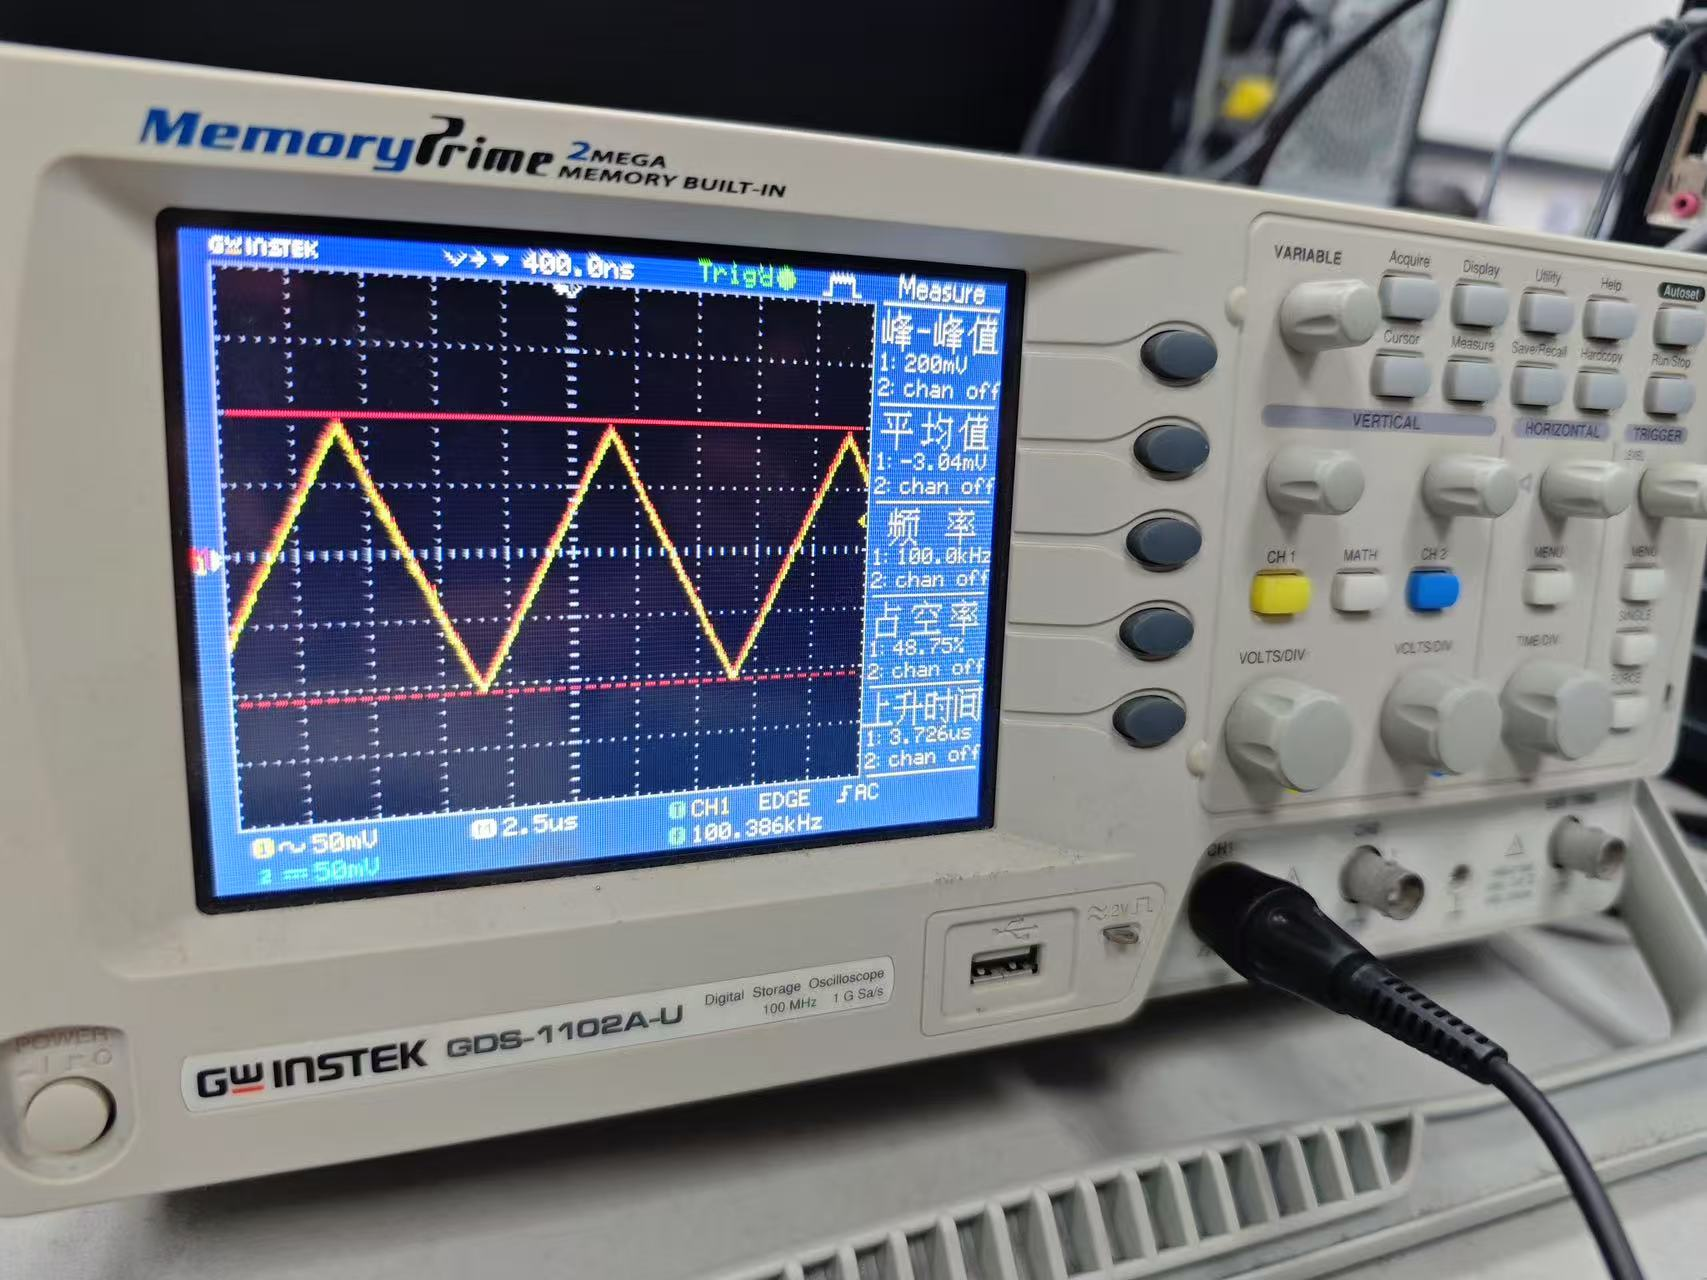
\includegraphics[width = .7\textwidth]{./figures/微信图片_20250318113547.jpg}
\caption{实验过程}
\end{figure}
通过设定不同的幅度,并用Cursor法测量信号幅度,并计算误差。
\begin{table}[H]
  \centering
  \caption{变化信号幅度}
  \begin{tabular}{C{.15\textwidth}C{.15\textwidth}C{.15\textwidth}C{.15\textwidth}C{.2\textwidth}}
  \toprule
  设定值  & Y1 & Y2 & Y1-Y2 & 误差分析 \\
  \midrule
  0.5Vp-p & 248mV & -264mV & 512mV & 2.40\% \\
  1Vp-p & 1.00V & -1.00V & 2.00V & 0.00\%\\
  1.5Vp-p & 736mV & -760mV & 1.49V & 0.67\% \\
  2.0Vp-p & 960mV & -1.05V & 2.01V & 0.50\% \\
  \bottomrule
  \end{tabular}
\end{table}
\section{电路板调试}
\subsection{呼吸灯调试}
\begin{table}[H]
  \centering
  \caption{呼吸灯不同引脚信号情况}
  \begin{tabular}{C{.15\textwidth}C{.15\textwidth}C{.15\textwidth}C{.2\textwidth}}
    \toprule
  引脚 & 波形  & 幅度    & 周期     \\
  \midrule
  1脚 & 三角波 & 2.72V & 1.200s \\
  7脚 & 方波  & 9.76V & 1.170s\\
  \bottomrule
  \end{tabular}
  \end{table}
初始时呼吸灯节奏最快,调整电位器R3,波形周期逐渐变长,频率变缓。
\subsection{幸运转盘调试}
\begin{table}[H]
\centering
\caption{幸运转盘信号情况}
\begin{tabular}{C{.15\textwidth}C{.15\textwidth}C{.15\textwidth}C{.2\textwidth}}
  \toprule
引脚    & 正/负脉冲宽度 & 幅度    & 周期    \\
\midrule
U1 3脚 & 72$\mu$ s & 4.00V & 20ms  \\
U2    & 17ms    & 2.01V & 170ms \\
\bottomrule
\end{tabular}
\end{table}
\begin{figure}[H]
  \centering
  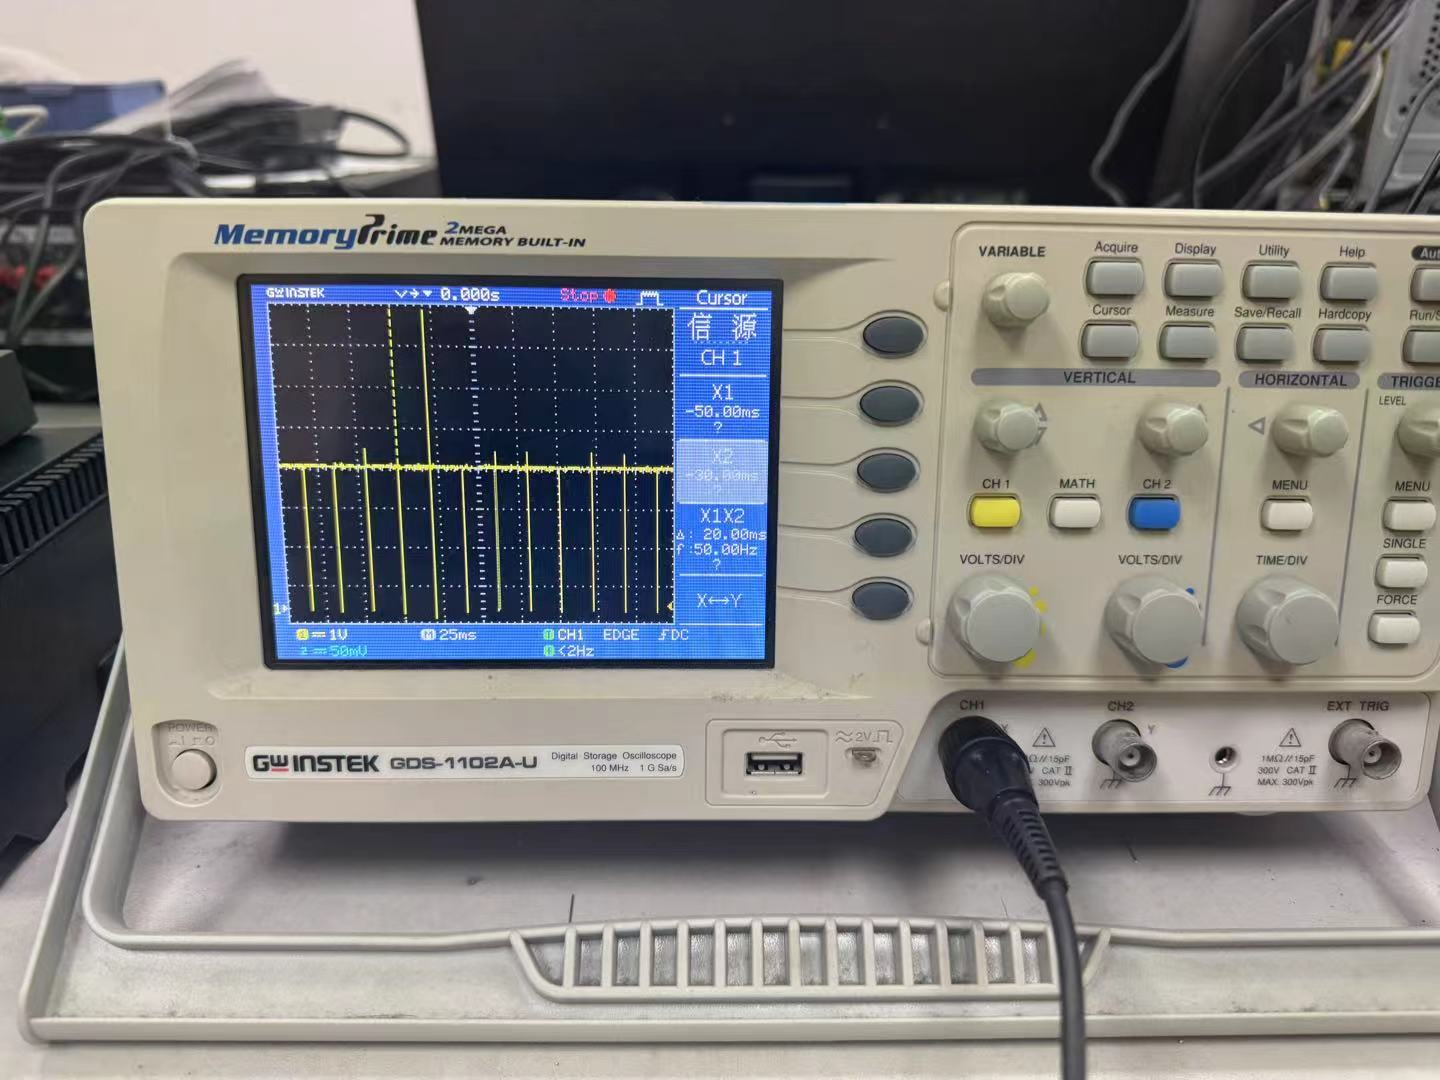
\includegraphics[width = .4\textwidth]{./figures/脉冲周期.jpg}
  \caption{负脉冲周期测量}
\end{figure}
计算U2芯片占空比=$\frac{\text{脉冲宽度}}{\text{周期}} = \frac{17\text{ms}}{170\text{ms}} = 10\%$

当灯停止闪烁时,三极管发射极电压约为2.40V。
\subsection{贴片流水灯调试}
\begin{table}[H]
\centering
\caption{555芯片输出信号的幅度频率及上升下降时间}
\begin{tabular}{C{.15\textwidth}C{.15\textwidth}C{.15\textwidth}C{.15\textwidth}C{.2\textwidth}}
  \toprule
引脚       & 幅度    & 周期      & 信号上升时间 & 信号下降时间 \\
\midrule
NE555 3脚 & 2.48V & 70.02ms & 120ns  & 164ns\\
\bottomrule
\end{tabular}
\end{table}
\begin{figure}[H]
  \centering
  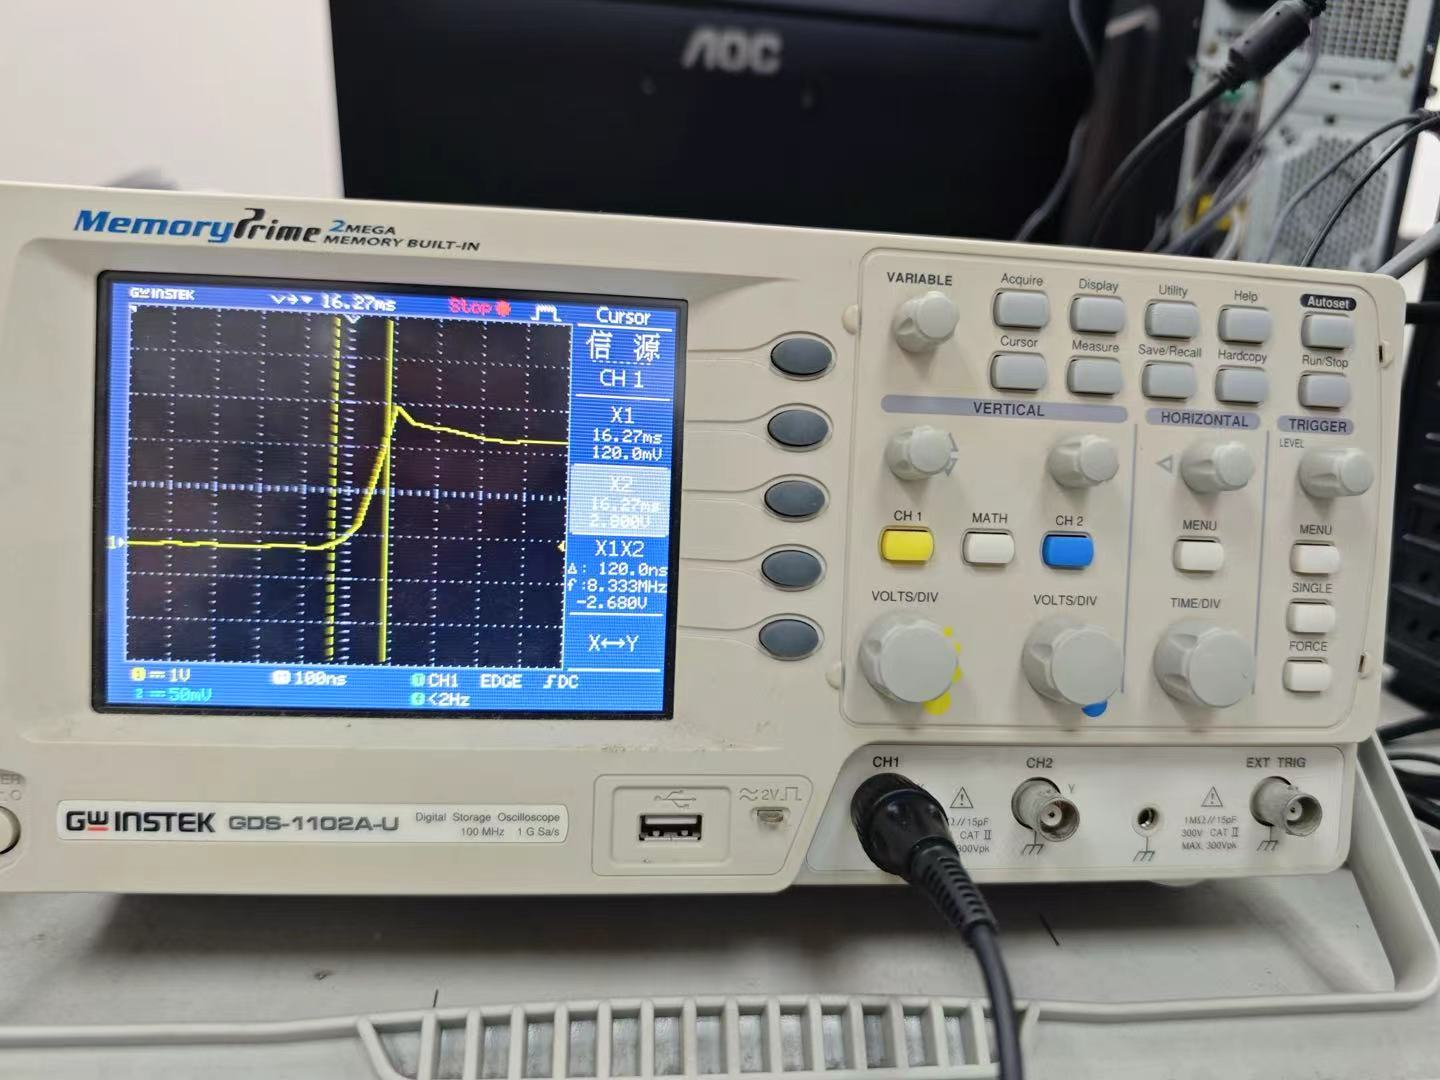
\includegraphics[width = .4\textwidth]{./figures/上升时间.jpg}
  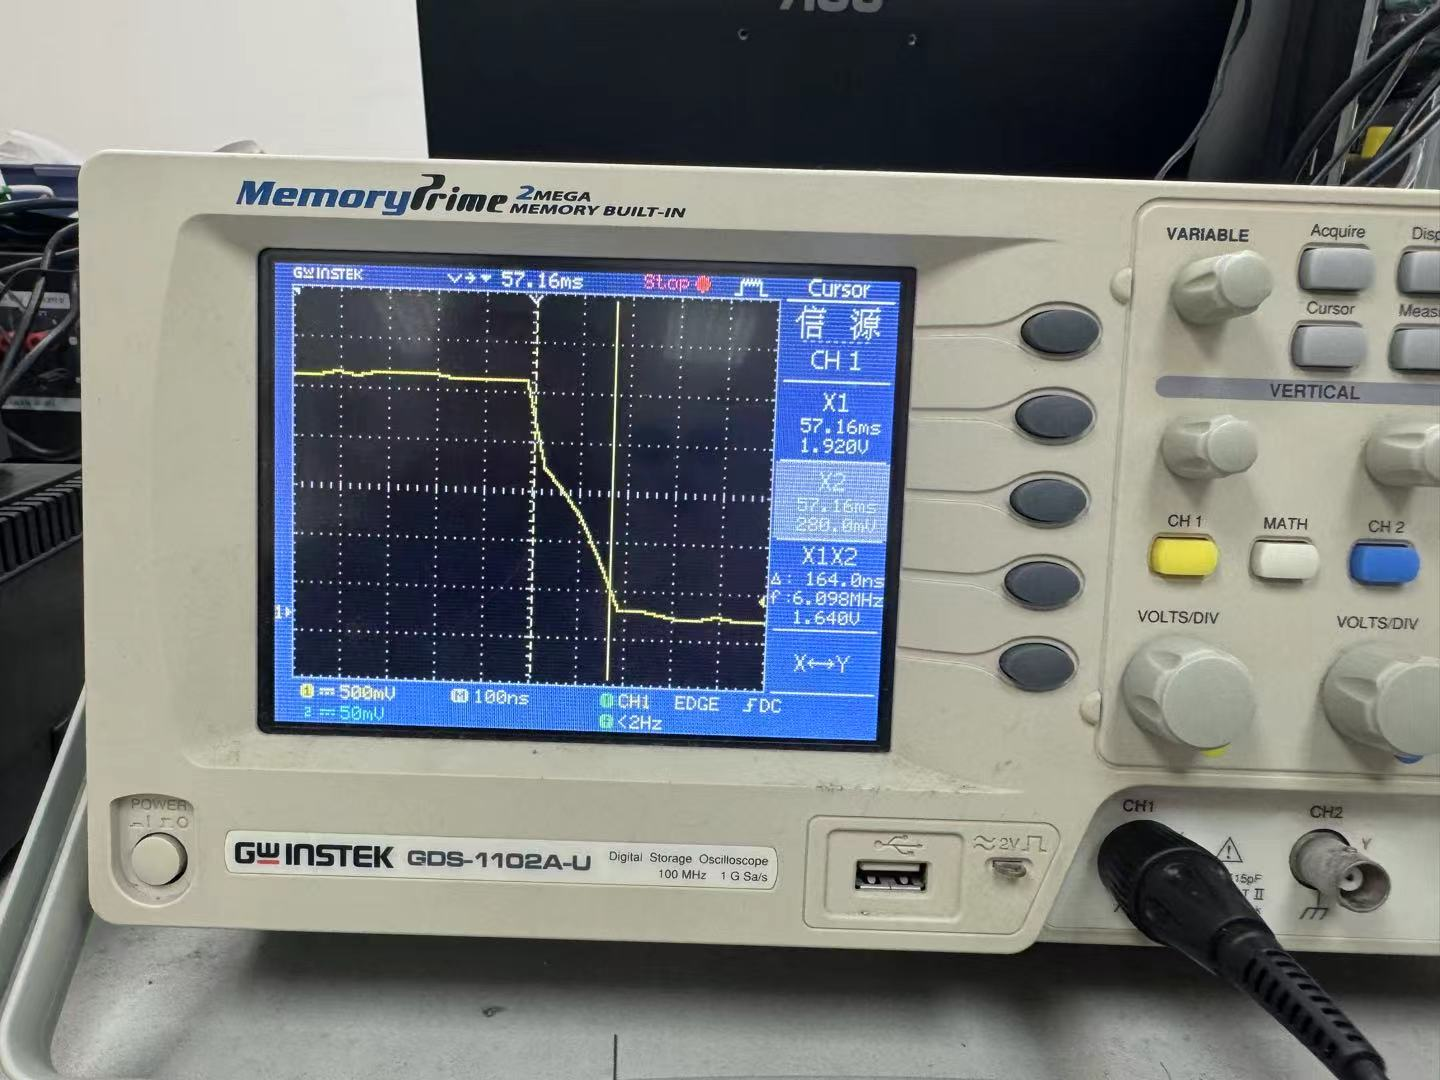
\includegraphics[width = .4\textwidth]{./figures/下降时间.jpg}
  \caption{信号上升下降时间的测量}
\end{figure}
\begin{table}[H]
\centering
\caption{环形计数器信号情况}
\begin{tabular}{C{.2\textwidth}C{.15\textwidth}C{.15\textwidth}C{.15\textwidth}C{.2\textwidth}}
  \toprule
引脚        & 周期    & 脉冲宽度 & 占空比    \\
\midrule
4017环形计数器 & 740ms & 70ms & 9.45\% \\
\bottomrule
\end{tabular}
\end{table}
理论占空比应为10\%。

Q1集电极周期:750ms。
\section{实验总结}
\subsection{实验收获}
本次实验涵盖内容广,包含了电子技术实践的许多基本方法。

在焊接过程中,我初步掌握了焊接的基本方法,也了解了贴片元器件的焊接。

第一部分常用电子仪器使用,让我掌握了万用表,电源,示波器等设备的基本使用方法,并且让我通过实践的方式测量了许多与电子技术实践相关的物理量,而且也通过误差分析让我了解到每个
电子元器件的差异。在示波器使用阶段,我测量了信号源的信号,并测量与计算了许多关于信号的物理量,而这一步操作也为我后面芯片调试打下基础。

第二部分电路板调试,我直观得了解到了芯片所发出信号的波形,并测量计算了信号的幅度,频率,占空比等,让我了解到了电路中信号的传输方法。
\subsection{对教学的建议}
整体而言电子工训这门课的基础实验环节安排十分得当,能够循序渐进的教会我许多电子电路焊接测量与调试的基本方法。

但是在教授的过程中往往出现大量的知识点,而先讲完全部知识点再实验的方法容易让我忘记一些知识点,而我认为一边讲解一边实践的方式可能会稍微好一些。

而且由于没有学习过电路设计的相关知识,流水灯,幸运转盘等电路的原理对我们来说都不太明朗,只能按照实验步骤完成实验,不能更好理解数据背后代表的含义。可能可以在课后增加答疑或资料补充,让我们更好理解电路的基本知识。
\end{document}